\documentclass[border=2mm]{standalone}
\usepackage{pgfplots}
\usepgfplotslibrary{groupplots}
\pgfplotsset{compat=1.18}
\definecolor{BCred}{rgb}{0.7, 0.11, 0.11}
\definecolor{BCblue}{rgb}{0.0, 0.20, 0.42}
\definecolor{BCgreen}{rgb}{0.11, 0.35, 0.02}
\pgfplotsset{every axis/.append style={
  width=7cm, height=7cm, scale only axis,
  ticklabel style={font=\scriptsize, /pgf/number format/fixed, /pgf/number format/precision=2},
  yticklabel style={text width=10mm, align=right},
  ylabel style={text width=10mm, align=center},
  label style={font=\small},
  title style={font=\small},
  legend style={draw=none, font=\footnotesize}}}
\begin{document}
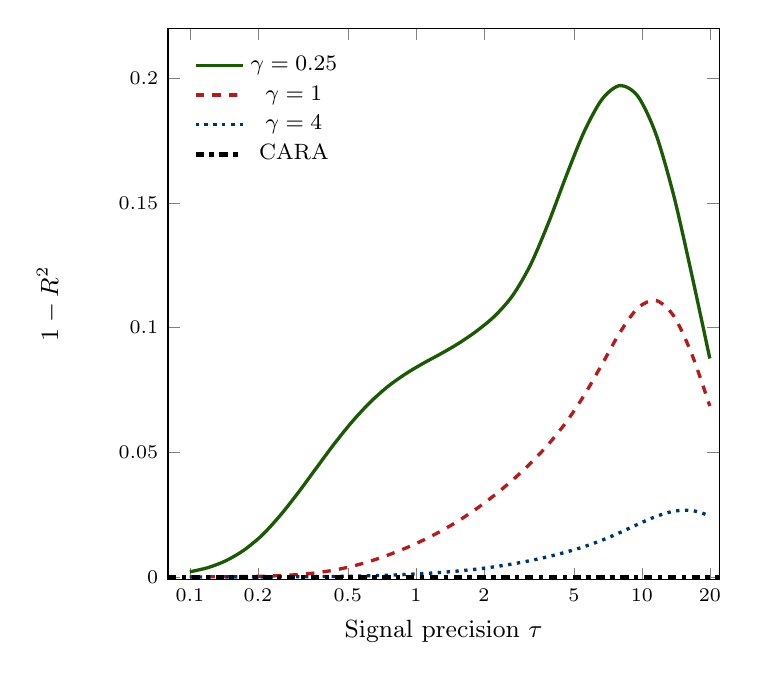
\begin{tikzpicture}
\begin{groupplot}[group style={group size=1 by 1}]
\nextgroupplot[scaled ticks=false,
  ymin=-0.001, ymax=0.22, ylabel={$1-R^2$},
  xmin=0.08, xmax=22, xmode=log,
  xlabel={Signal precision $\tau$},
  xtick={0.1,0.2,0.5,1,2,5,10,20},
  xticklabels={0.1,0.2,0.5,1,2,5,10,20},
  legend pos=north west]
% gamma=0.25 (REAL DATA from solver, G=15)
\addplot[very thick,color=BCgreen,smooth] coordinates {(0.1,0.00205)(0.120,0.00371)(0.144,0.00645)(0.173,0.01066)(0.208,0.01660)(0.249,0.02429)(0.299,0.03334)(0.359,0.04310)(0.431,0.05283)(0.518,0.06185)(0.622,0.06966)(0.746,0.07610)(0.896,0.08128)(1.075,0.08558)(1.291,0.08949)(1.549,0.09368)(1.860,0.09862)(2.233,0.10460)(2.681,0.11282)(3.218,0.12515)(3.863,0.14196)(4.637,0.16096)(5.567,0.17865)(6.683,0.19164)(8.022,0.19702)(9.630,0.19258)(11.561,0.17740)(13.878,0.15253)(16.660,0.12095)(20.0,0.08757)};
% gamma=1.0 (REAL DATA)
\addplot[very thick,color=BCred,dashed,smooth] coordinates {(0.1,0.00002)(0.120,0.00004)(0.144,0.00007)(0.173,0.00014)(0.208,0.00027)(0.249,0.00051)(0.299,0.00092)(0.359,0.00161)(0.431,0.00266)(0.518,0.00418)(0.622,0.00618)(0.746,0.00862)(0.896,0.01145)(1.075,0.01468)(1.291,0.01836)(1.549,0.02259)(1.860,0.02741)(2.233,0.03283)(2.681,0.03886)(3.218,0.04557)(3.863,0.05320)(4.637,0.06217)(5.567,0.07293)(6.683,0.08541)(8.022,0.09815)(9.630,0.10793)(11.561,0.11083)(13.878,0.10447)(16.660,0.08922)(20.0,0.06851)};
% gamma=4.0 (REAL DATA)
\addplot[very thick,color=BCblue,dotted,smooth] coordinates {(0.1,0.00000)(0.120,0.00000)(0.144,0.00001)(0.173,0.00001)(0.208,0.00002)(0.249,0.00003)(0.299,0.00006)(0.359,0.00011)(0.431,0.00018)(0.518,0.00029)(0.622,0.00045)(0.746,0.00067)(0.896,0.00096)(1.075,0.00133)(1.291,0.00180)(1.549,0.00239)(1.860,0.00314)(2.233,0.00407)(2.681,0.00521)(3.218,0.00656)(3.863,0.00815)(4.637,0.00999)(5.567,0.01216)(6.683,0.01476)(8.022,0.01783)(9.630,0.02116)(11.561,0.02424)(13.878,0.02635)(16.660,0.02664)(20.0,0.02452)};
% CARA
\addplot[ultra thick,color=black,dashdotted] coordinates {(0.08,0)(22,0)};
\legend{$\gamma = 0.25$, $\gamma = 1$, $\gamma = 4$, CARA}
\end{groupplot}
\end{tikzpicture}
\end{document}
